\begin{frame}
%	\frametitle{References}
%\BgThispage


\vspace{3cm}
\centering
\Huge \textcolor{black}{Questions?}\\[1cm]
\begin{figure}
     \includegraphics[scale=0.21]{Resources/Images/imagesThesis/presentation_swe_of_sup47}
     \end{figure}
%	\centering
%	$\rightarrow$ to optimally use the network, adaptive scheduling policy is required
	
%	\footnotetext[1]{derived numerically}
	
\end{frame}
\clearpage




%%%%%%%%%%%%%%%%%%%%
%%%%%%%%%%%%%%%%%%%%
\begin{frame}
    \shiftedframetitle{2. Theory -  \large Shallow Water Equations  model {\small(cont)}}
%\vspace{-2mm}
%\begin{columns}
\begin{minipage}{0.35\textwidth}
\begin{itemize}
\item<1->[] SWE model can be represented as a matrix form \dots
% derived from mass and momentum conservation laws, and depth averaging \dots %also derived by vertical averaging from the 3d incompressible ns eqs
\item<1->[]
\begin{align*}
\vspace{-15pt}
&\begin{bmatrix}[1.3]
\myTUMdarkblue{h}\\
\myTUMdarkblue{hu}\\
\myTUMdarkblue{hv}\\
\end{bmatrix}_t \ + \
\begin{bmatrix}[1.0]
hu\\
hu^2 + \frac{1}{2}gh^2\\
huv\\
\end{bmatrix}_x\ + \
\begin{bmatrix}[1.0]
hv\\
huv\\
hv^2 + \frac{1}{2}gh^2\\
\end{bmatrix}_y =
\begin{bmatrix}[1.0]
0\\
-gh\ b_x\\
-gh\ b_y
\end{bmatrix}\\[2em]
%&\bar{q} = \begin{bmatrix}[1.3]
%\myTUMdarkblue{h}\\
%\myTUMdarkblue{hu}\\
%\myTUMdarkblue{hv}
%\end{bmatrix}
%\begin{matrix}[1.0]
%\text{\hspace{-3em}\myTUMdarkblue{$\rightarrow\ $\textit{height}}}\\
%\text{\hspace{-2pt}\myTUMdarkblue{$\rightarrow\ $\textit{discharge in x}}} \\
%\text{\hspace{5pt}\myTUMdarkblue{$\rightarrow\ $\textit{discharge in y}}}
%\end{matrix}
&\qquad \lambda^x = 
\begin{bmatrix}[1.0]
u - c\\
u\\
u+c
\end{bmatrix}
,\qquad  \lambda^y = 
\begin{bmatrix}[1.0]
v - c\\
v\\
v+c
\end{bmatrix}
,\qquad c = \sqrt{gh}
\end{align*}
\item<1->[]
\begin{align*}
\qquad \qquad \frac{\partial \myTUMdarkblue{\bar{q}}}{\partial t} + \dfrac{\partial F(\myTUMdarkblue{\bar{q}})}{\partial x} + &\frac{\partial G(\myTUMdarkblue{\bar{q}})}{\partial y} = S(h,x,y,t)
\end{align*}
\end{itemize}
\end{minipage}
\begin{minipage}{0.45\textwidth}  
\begin{itemize}[leftmargin=*]
\item<1->[]
\vspace{2cm}
\begin{center}
\begin{figure}
\includegraphics[width=\textwidth]{./Resources/Images/imagesThesis/floor.png}
\label{fig:swechemedit}
\end{figure}
\end{center}
\end{itemize}
\end{minipage}

\end{frame}
\clearpage


%%%%%%%%%%%%%%%%
%%%%%%%%%%%%%%%%
\begin{frame}
    \shiftedframetitle{2. Theory - \large Flow characterization \small(final)}
\begin{minipage}{0.5\textwidth}
\vspace{1cm}
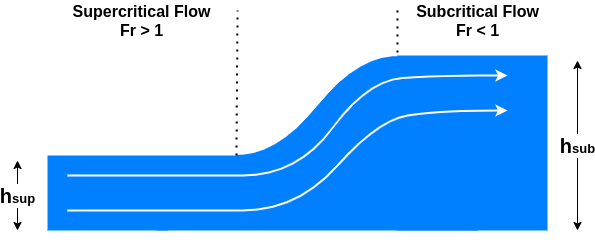
\includegraphics[width=\textwidth]{Resources/Images/imagesThesis/hydjump2.png}
\end{minipage}
\hspace{1cm}
\begin{minipage}{0.4\textwidth}
\vspace{1.5cm}
\begin{tcolorbox}[colback=white] 
\begin{itemize}
\setlength{\itemsep}{1cm}
\item[] $\mathbf{Fr = \dfrac{V}{c} =\dfrac{V}{\sqrt{gh}} \propto \dfrac{inertia\ force}{gravity\ force}}$
\item Supercritical $\sqrt{gh}\ < V$
\item Subcritical $\sqrt{gh}\ > V$
\item Critical $\sqrt{gh}\  =  V$
\end{itemize}
\end{tcolorbox}
\end{minipage}
\end{frame}
